% 第二部分：GRPO 训练结果（由 main_zh.tex 引入）。

\section{评判模型能为验证器带来增益吗？}\label{sec:res-grpo}

\subsection{学习率}\label{sec:res-sweep}

学习率只在验证集上选一次，使用 \texttt{rlvr} 奖励和种子 1。每个扫描 run 训练 60 步，每步 16 道题、每题 8 个回答，学习率分别为 $10^{-5}$、$3\cdot10^{-5}$ 和 $10^{-4}$（表~\ref{tab:sweep}）。选择规则是：取第 30 步和第 60 步验证准确率均值最高的学习率；若最好的两个相差不超过 0.5 个百分点，则取较小的那个（\file{experiments/part2_llm/LR_SELECTION.md}）。这条规则是在 $10^{-5}$ 和 $10^{-4}$ 两个 run 刚开始时写下的；当时 $3\cdot10^{-5}$ 的 run 已经记录了第 0 步和第 30 步的准确率，我们也看过。$10^{-5}$（\NUM{sweep_1em5_score}）与 $3\cdot10^{-5}$（\NUM{sweep_3em5_score}）相差不超过 0.5 个百分点，因此规则为第二、三部分的所有 run 选定了 $10^{-5}$。在 $10^{-4}$ 下，验证准确率到第 30 步升至 \NUM{sweep_1em4_30}，到第 60 步又跌到 \NUM{sweep_1em4_60}，低于基座模型。三个 run 都从同一个基座模型出发，第 0 步的准确率却不同（\NUM{sweep_1em5_0}、\NUM{sweep_3em5_0}、\NUM{sweep_1em4_0}）：vLLM 上的贪心解码在不同服务器状态下并非逐位可复现，这一差异就是评估噪声的大小。

\begin{table}[t]
\centering\small
\begin{tabular}{@{}lcccc@{}}
\toprule
学习率 & 第 0 步 & 第 30 步 & 第 60 步 & 得分（第 30 与 60 步均值） \\ \midrule
$10^{-5}$ & \NUM{sweep_1em5_0} & \NUM{sweep_1em5_30} & \NUM{sweep_1em5_60} & \NUM{sweep_1em5_score} \\
$3\cdot10^{-5}$ & \NUM{sweep_3em5_0} & \NUM{sweep_3em5_30} & \NUM{sweep_3em5_60} & \NUM{sweep_3em5_score} \\
$10^{-4}$ & \NUM{sweep_1em4_0} & \NUM{sweep_1em4_30} & \NUM{sweep_1em4_60} & \NUM{sweep_1em4_score} \\
\bottomrule
\end{tabular}
\caption{学习率扫描：\texttt{rlvr}、种子 1 的验证准确率（500 道留出的 MATH 训练题，贪心解码）。}
\label{tab:sweep}
\end{table}

\subsection{奖励条件}\label{sec:res-cond}

\texttt{rlvr} 和 \texttt{rlvr\_kev\_add} 各跑了 \NUM{seeds_rlvr} 个种子，其余条件各 \NUM{seeds_kevgate} 个。表~\ref{tab:grpo-acc} 给出最终策略的准确率，表~\ref{tab:grpo-seeds} 给出每个 run 的准确率，表~\ref{tab:grpo-paired} 给出相对 \texttt{rlvr} 的配对差，图~\ref{fig:grpo-curves} 给出训练曲线。配对区间按题目重采样，不包含种子之间的差异；而在这些 run 中，种子之间的差异才是更大的那一个。

\paragraph{只用验证器。} \texttt{rlvr} 训练 200 步，把 MATH-500 从 \NUM{acc_base_math}\%（基座模型）提高到 \NUM{acc_rlvr_math}\%，GSM8K 从 \NUM{acc_base_gsm}\% 提高到 \NUM{acc_rlvr_gsm}\%，AMC23 从 \NUM{acc_base_amc}\% 提高到 \NUM{acc_rlvr_amc}\%，AIME24 和 AIME25 从 \NUM{acc_base_aime24}\% 和 \NUM{acc_base_aime25}\% 提高到 \NUM{acc_rlvr_aime24}\% 和 \NUM{acc_rlvr_aime25}\%。

\begin{table}[t]
\centering\small
\begin{tabular}{@{}lcccccc@{}}
\toprule
condition & seeds & MATH-500 & GSM8K & AMC23 & AIME24 & AIME25 \\ \midrule
base model & -- & 76.5 & 87.9 & 50.6 & 10.0 & 10.9 \\ \midrule
\texttt{rlvr} & 3 & 82.5 $\pm$ 0.6 & 93.0 $\pm$ 0.3 & 60.9 $\pm$ 2.4 & 21.5 $\pm$ 0.4 & 16.7 $\pm$ 2.1 \\
\texttt{rlvr\_kev\_add} & 3 & 84.6 $\pm$ 2.6 & 93.1 $\pm$ 0.9 & 65.6 $\pm$ 3.9 & 25.6 $\pm$ 6.6 & 18.6 $\pm$ 5.5 \\
\texttt{rlvr\_kev\_gate} & 2 & 85.2 $\pm$ 4.5 & 93.3 $\pm$ 0.5 & 67.7 $\pm$ 4.6 & 28.5 $\pm$ 8.5 & 21.1 $\pm$ 4.9 \\
\texttt{kev\_only} & 2 & 70.7 $\pm$ 1.3 & 91.3 $\pm$ 0.0 & 41.8 $\pm$ 2.3 & 4.9 $\pm$ 1.0 & 2.3 $\pm$ 1.5 \\
\texttt{rlvr\_ar\_add} & 2 & 82.4 $\pm$ 1.7 & 93.2 $\pm$ 0.8 & 62.1 $\pm$ 2.3 & 21.6 $\pm$ 2.8 & 18.0 $\pm$ 1.9 \\
\bottomrule
\end{tabular}

\caption{最终策略：准确率（\%），种子均值 $\pm$ 种子间标准差。MATH-500 和 GSM8K（1319 题）：贪心解码。AMC23、AIME24 和 AIME25：温度 0.6 下每题 16 个样本的平均。基座模型：两次评估的平均。}
\label{tab:grpo-acc}
\end{table}

\begin{table}[t]
\centering\small
\begin{tabular}{@{}lcccccc@{}}
\toprule
condition & seed & MATH-500 & GSM8K & AMC23 & AIME24 & AIME25 \\ \midrule
\texttt{rlvr} & 1 & 82.8 & 93.0 & 63.6 & 21.0 & 18.8 \\
 & 2 & 83.0 & 93.3 & 59.8 & 21.9 & 16.9 \\
 & 3 & 81.8 & 92.6 & 59.2 & 21.7 & 14.6 \\
\addlinespace
\texttt{rlvr\_kev\_add} & 1 & 82.2 & 92.1 & 62.5 & 21.9 & 13.8 \\
 & 2 & 84.2 & 93.6 & 64.4 & 21.7 & 17.5 \\
 & 3 & 87.4 & 93.7 & 70.0 & 33.1 & 24.6 \\
\addlinespace
\texttt{rlvr\_kev\_gate} & 1 & 82.0 & 92.9 & 64.4 & 22.5 & 17.7 \\
 & 2 & 88.4 & 93.7 & 70.9 & 34.6 & 24.6 \\
\addlinespace
\texttt{kev\_only} & 1 & 69.8 & 91.3 & 40.2 & 4.2 & 1.2 \\
 & 2 & 71.6 & 91.3 & 43.4 & 5.6 & 3.3 \\
\addlinespace
\texttt{rlvr\_ar\_add} & 1 & 81.2 & 92.6 & 60.5 & 19.6 & 16.7 \\
 & 2 & 83.6 & 93.8 & 63.7 & 23.5 & 19.4 \\
\bottomrule
\end{tabular}

\caption{每个 run 的最终策略：准确率（\%），口径同表~\ref{tab:grpo-acc}。}
\label{tab:grpo-seeds}
\end{table}

\paragraph{每个 \kev{} 条件都有一个种子遥遥领先。} \texttt{rlvr} 的三个种子在 MATH-500 上最终为 \NUM{acc_rlvr_math_s1}\%、\NUM{acc_rlvr_math_s2}\% 和 \NUM{acc_rlvr_math_s3}\%，在 AIME24 上为 \NUM{acc_rlvr_aime24_s1}\%、\NUM{acc_rlvr_aime24_s2}\% 和 \NUM{acc_rlvr_aime24_s3}\%（表~\ref{tab:grpo-seeds}）。把 \kev{} 的 $\pc$ 加入奖励后，两个种子的结果与之相近（MATH-500 上 \NUM{acc_kevadd_math_s1}\% 和 \NUM{acc_kevadd_math_s2}\%），第三个为 \NUM{acc_kevadd_math_s3}\%。用门控时，一个种子为 \NUM{acc_kevgate_math_s1}\%，另一个为 \NUM{acc_kevgate_math_s2}\%。在 AIME24 上，这两个领先的种子达到 \NUM{acc_kevadd_aime24_s3}\% 和 \NUM{acc_kevgate_aime24_s2}\%，本文其他 run 都不超过 \NUM{potheraime24max}\%。这两个 run 撑起了各自条件的均值，也撑起了相对 \texttt{rlvr} 的配对差：\texttt{rlvr\_kev\_add} 在 MATH-500 上为 \NUM{d_kevadd_math} \ci{\NUM{dlo_kevadd_math}}{\NUM{dhi_kevadd_math}} 个百分点，\texttt{rlvr\_kev\_gate} 为 \NUM{d_kevgate_math} \ci{\NUM{dlo_kevgate_math}}{\NUM{dhi_kevgate_math}}，在竞赛题集上更大（表~\ref{tab:grpo-paired}）。这些区间说明，在这些题目上这两个条件的种子均值高于 \texttt{rlvr}；它们并不说明差别来自评判模型：同一条件的其他种子并没有超过 \texttt{rlvr}。加入 AR 评判模型的 $P_{\mathrm{a}}$（\texttt{rlvr\_ar\_add}）时，两个种子都与 \texttt{rlvr} 相近（MATH-500 上 \NUM{d_aradd_math} \ci{\NUM{dlo_aradd_math}}{\NUM{dhi_aradd_math}} 个百分点）。让这两个领先 run 与众不同的，是它们的写法（\S\ref{sec:res-style}）。

\begin{table}[t]
\centering\small
\begin{tabular}{@{}lccccc@{}}
\toprule
minus \texttt{rlvr} & MATH-500 & GSM8K & AMC23 & AIME24 & AIME25 \\ \midrule
\texttt{rlvr\_kev\_add} & $+$2.1 & $+$0.1 & $+$4.7 & $+$4.0 & $+$1.9 \\
 & {\footnotesize \ci{0.6}{3.6}} & {\footnotesize \ci{$-$0.5}{0.8}} & {\footnotesize \ci{1.6}{8.2}} & {\footnotesize \ci{0.1}{8.3}} & {\footnotesize \ci{0.2}{3.7}} \\[2pt]
\texttt{rlvr\_kev\_gate} & $+$2.7 & $+$0.3 & $+$6.8 & $+$7.0 & $+$4.4 \\
 & {\footnotesize \ci{0.7}{4.8}} & {\footnotesize \ci{$-$0.4}{1.0}} & {\footnotesize \ci{2.6}{11.3}} & {\footnotesize \ci{2.4}{12.2}} & {\footnotesize \ci{1.3}{8.2}} \\[2pt]
\texttt{kev\_only} & $-$11.8 & $-$1.7 & $-$19.1 & $-$16.6 & $-$14.4 \\
 & {\footnotesize \ci{$-$14.6}{$-$9.1}} & {\footnotesize \ci{$-$2.6}{$-$0.9}} & {\footnotesize \ci{$-$28.2}{$-$10.4}} & {\footnotesize \ci{$-$26.9}{$-$7.5}} & {\footnotesize \ci{$-$24.4}{$-$5.9}} \\[2pt]
\texttt{rlvr\_ar\_add} & $-$0.1 & $+$0.2 & $+$1.2 & $+$0.0 & $+$1.3 \\
 & {\footnotesize \ci{$-$1.9}{1.6}} & {\footnotesize \ci{$-$0.5}{0.9}} & {\footnotesize \ci{$-$2.0}{4.7}} & {\footnotesize \ci{$-$2.5}{3.0}} & {\footnotesize \ci{$-$1.6}{4.6}} \\[2pt]
\bottomrule
\end{tabular}

\caption{相对 \texttt{rlvr} 的配对差（百分点）：逐题取各条件的种子均值之差，再对题目取平均，附按题目自助法得到的 95\% 区间。}
\label{tab:grpo-paired}
\end{table}

\paragraph{只用评判模型会被钻空子。} 没有验证器时（\texttt{kev\_only}），策略最大化 \kev{} 的 $\pc$：在最后 20 步的训练解答上，它升到 \NUM{kevc_kevonly}（\texttt{rlvr}：\NUM{kevc_rlvr}），而验证器在同样这些解答上的准确率停在 \NUM{trainacc_kevonly}\%（\texttt{rlvr}：\NUM{trainacc_rlvr}\%）。与 \texttt{rlvr} 相比，最终策略在 MATH-500 上相差 \NUM{d_kevonly_math} \ci{\NUM{dlo_kevonly_math}}{\NUM{dhi_kevonly_math}} 个百分点，在 AIME24 上相差 \NUM{d_kevonly_aime24}；两个种子在 MATH-500 上都低于它们出发时的基座模型（\NUM{acc_kevonly_math_s1}\% 和 \NUM{acc_kevonly_math_s2}\%，基座为 \NUM{acc_base_math}\%），在三个竞赛题集上也都如此。策略学会的是写出 \kev{} 认为正确的解答：\kev{} 给它在 MATH-500 上的错误答案平均打 \NUM{skevwrong_kevonly}，而给 \texttt{rlvr} 各策略的错误答案打 \NUM{skevwrong_rlvr}。\kev{} 在训练解答上的组内 AUROC——GRPO 的优势用的正是组内比较——从前 20 步的 \NUM{kevaucwtr_first20_kevonly} 降到最后 20 步的 \NUM{kevaucwtr_last20_kevonly}。对于没有针对它做优化的策略，4B 的评判模型是可用的信号（\S\ref{sec:res-study}）；单独作为奖励，它不可用。

\begin{table}[t]
\centering\small
\begin{tabular}{@{}lccccccc@{}}
\toprule
 & \multicolumn{5}{c}{training, last 20 steps} & \multicolumn{2}{c}{final policy, MATH-500} \\ \cmidrule(lr){2-6}\cmidrule(l){7-8}
condition & accuracy & \kev{} $\pc$ & tokens & all wrong & all right & \kev{} $\pc$ & \kev{} AUROC \\ \midrule
\texttt{rlvr} & 67.0 & 0.74 & 679 & 16\% & 44\% & 0.81 & 0.88 \\
\texttt{rlvr\_kev\_add} & 69.0 & 0.74 & 593 & 14\% & 46\% & 0.82 & 0.89 \\
\texttt{rlvr\_kev\_gate} & 69.7 & 0.78 & 831 & 14\% & 47\% & 0.87 & 0.89 \\
\texttt{kev\_only} & 55.5 & 0.87 & 829 & 25\% & 32\% & 0.91 & 0.85 \\
\texttt{rlvr\_ar\_add} & 68.0 & 0.73 & 585 & 15\% & 47\% & 0.80 & 0.89 \\
\bottomrule
\end{tabular}

\caption{最后 20 步的训练统计（种子均值）：训练解答的验证器准确率、每步其中 64 个解答上 \kev{} 的平均 $\pc$、解答词元数，以及组内解答全错或全对（验证器不给学习信号）的组所占比例。最终策略：MATH-500 解答上 \kev{} 的平均 $\pc$ 及其对验证结果的 AUROC。}
\label{tab:grpo-train}
\end{table}

\begin{figure}[t]
\centering
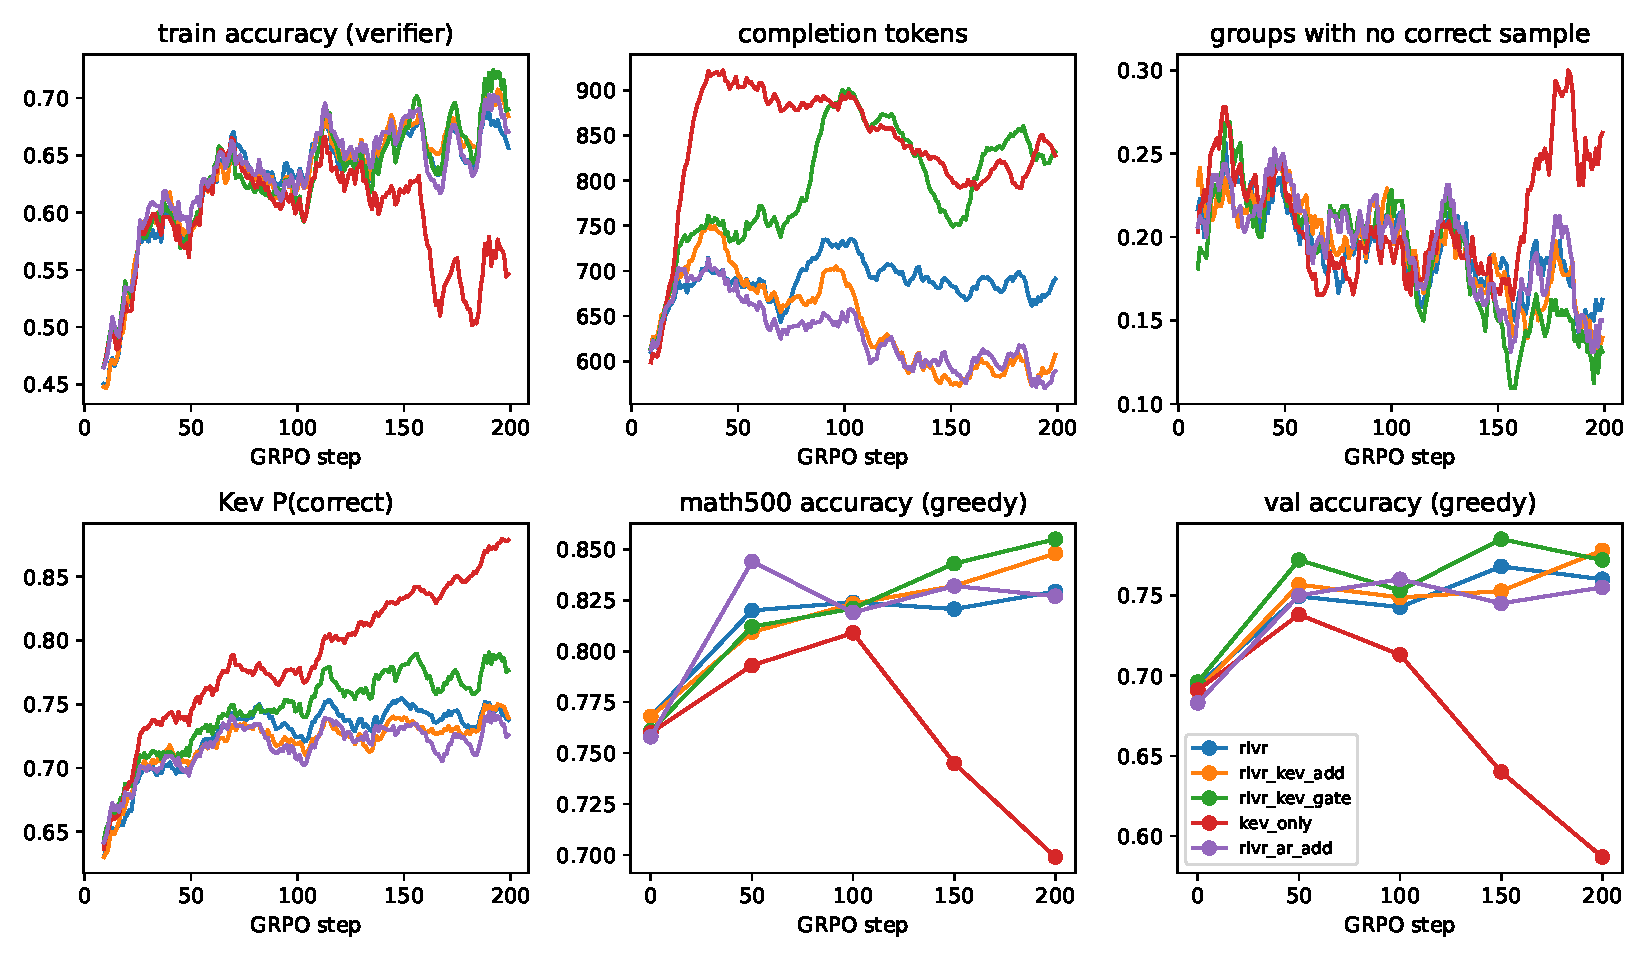
\includegraphics[width=\linewidth]{../../experiments/part2_llm/results/training_curves.pdf}
\caption{训练曲线（种子均值）：训练解答的验证器准确率、解答词元数、没有任何正确解答的组所占比例、训练解答上 \kev{} 的 $\pc$（10 步滑动平均），以及每 50 步在 MATH-500 和验证集上的贪心准确率。}
\label{fig:grpo-curves}
\end{figure}

\paragraph{评估噪声。} 每个 run 都在第 0 步评估基座模型。在 \NUM{szruns_math500} 个 run 中，第 0 步的 MATH-500 准确率在 \NUM{szmin_math500}\% 到 \NUM{szmax_math500}\% 之间（标准差 \NUM{szsd_math500} 个百分点），验证准确率在 \NUM{szmin_val}\% 到 \NUM{szmax_val}\% 之间。每个 run 的最终权重在 MATH-500 上被贪心评估两次：一次是第 200 步的定期评估，一次是最终评估。两次结果平均相差 \NUM{rptabs_math500} 个百分点，最多相差 \NUM{rptmax_math500}（\NUM{rptruns_math500} 个 run）。两个最终策略之间一个百分点的差异落在这一噪声之内；领先种子与其他种子之间的差异则不然。

\subsection{写解答的三种方式}\label{sec:res-style}

图~\ref{fig:style-example} 给出三个 run 的最终策略对同一道 MATH-500 题目的解答。多数策略写一份带 LaTeX 和 markdown 格式的解答，以框出的答案结尾（左）。两个领先的种子先用纯文本、不带 LaTeX 或 markdown 把题目做一遍，给出答案，多数情况下再写格式化的解答（中）。还有一些策略写完格式化的解答、给出答案之后，又用几乎相同的话把解答再写一遍（右）。第一种风格，我们用以非正式草稿开头的解答所占比例来衡量：前 300 个字符中没有数学定界符（\texttt{\$}、\texttt{\textbackslash(} 或 \texttt{\textbackslash[}），也没有 markdown 标题或粗体（\texttt{\#\#\#} 或 \texttt{**}）。第三种风格，我们用一个解答中（至少 20 个字符的）行有多大比例与该解答前面某行相同来衡量。这两个量都是在读过最终解答之后为了描述所见而定义的。

\begin{figure}[t]
\centering
\begin{minipage}[t]{0.31\linewidth}\raggedright\fontsize{6.5}{7.6}\selectfont\ttfamily
 We are given:\\
\mbox{}\\
- 5 shirts\\
- 6 pairs of pants\\
- 8 hats\\
\mbox{}\\
To make an outfit, we choose **one shirt**, **one pair of pants**, and **one hat**.\\
\mbox{}\\
Since the choices are independent, we multiply the number of options for each category:\\
\mbox{}\\
\$\$\\
5 \textbackslash{}times 6 \textbackslash{}times 8 = 240\\
\$\$\\
\mbox{}\\
So, the total number of possible outfits is:\\
\mbox{}\\
\$\$\\
\textbackslash{}boxed\{240\}\\
\$\$
\end{minipage}
\hfill
\begin{minipage}[t]{0.31\linewidth}\raggedright\fontsize{6.5}{7.6}\selectfont\ttfamily
 We have 5 shirts, 6 pairs of pants, and 8 hats. For each outfit, we choose one shirt, one pair of pants, and one hat. The total number of outfits is the product: 5 * 6 * 8 = 240.\\
\mbox{}\\
Thus, the answer is \textbackslash{}boxed\{240\}.\\
\mbox{}\\
To determine the total number of outfits consisting of one shirt, one pair of pants, and one hat, we use the fundamental counting principle.\\
\mbox{}\\
- There are 5 choices for shirts.\\
- There are 6 choices for pants.\\
- There are 8 choices for hats.\\
\mbox{}\\
Multiplying these together gives the total number of combinations:\\
\mbox{}\\
\textbackslash{}[\\
5 \textbackslash{}times 6 \textbackslash{}times 8 = 240\\
\textbackslash{}]\\
\mbox{}\\
Thus, the total number of possible outfits is:\\
\mbox{}\\
\textbackslash{}[\\
\textbackslash{}boxed\{240\}\\
\textbackslash{}]
\end{minipage}
\hfill
\begin{minipage}[t]{0.31\linewidth}\raggedright\fontsize{6.5}{7.6}\selectfont\ttfamily
 To determine the total number of outfits that can be made, we use the **fundamental counting principle**, which states that if there are multiple independent choices to be made, the total number of combinations is the product of the number of options for each choice.\\
\mbox{}\\
---\\
\mbox{}\\
\#\#\# Step-by-step Breakdown:\\
\mbox{}\\
- **Shirts**: 5 options\\
- **Pants**: 6 options\\
- **Hats**: 8 options\\
\mbox{}\\
Each outfit consists of **one shirt**, **one pair of pants**, and **one hat**, and each choice is independent of the others.\\
\mbox{}\\
---\\
\mbox{}\\
\#\#\# Total Outfits:\\
\mbox{}\\
\$\$\\
5 \textbackslash{}times 6 \textbackslash{}times 8 = 240\\
\$\$\\
\mbox{}\\
---\\
\mbox{}\\
\#\#\# Final Answer:\\
\mbox{}\\
\$\$\\
\textbackslash{}boxed\{240\}\\
\$\$\\
\mbox{}\\
We are given:\\
\mbox{}\\
- 5 shirts\\
- 6 pairs of pants\\
- 8 hats\\
\mbox{}\\
Each outfit consists of **one shirt**, **one pair of pants**, and **one hat**.\\
\mbox{}\\
---\\
\mbox{}\\
\#\#\# Step 1: Use the Fundamental Counting Principle\\
\mbox{}\\
Since each choice is independent, the total number of outfits is the product of the number of choices for each item:\\
\mbox{}\\
\$\$\\
5 \textbackslash{}times 6 \textbackslash{}times 8\\
\$\$\\
\mbox{}\\
---\\
\mbox{}\\
\#\#\# Step 2: Perform the Multiplication\\
\mbox{}\\
\$\$\\
5 \textbackslash{}times 6 = 30\\
\$\$\\
\$\$\\
30 \textbackslash{}times 8 = 240\\
\$\$\\
\mbox{}\\
---\\
\mbox{}\\
\#\#\# Final Answer:\\
\mbox{}\\
\$\$\\
\textbackslash{}boxed\{240\}\\
\$\$
\end{minipage}

\caption{一道 MATH-500 题目（\texttt{test/prealgebra/307}）上三个第二部分 run 的最终贪心解答，逐字照录（连续空行已缩短）。左：\texttt{rlvr} 种子 1（\NUM{exmtok_rlvr_s1} 个词元）。中：\texttt{rlvr\_kev\_gate} 种子 2，先写草稿（\NUM{exmtok_kevgate_s2} 个词元）。右：\texttt{rlvr} 种子 3，重复自己（\NUM{exmtok_rlvr_s3} 个词元）。三个解答都正确。选这道题只为举例：三个 run 都做对了，解答较短，而且只含 ASCII 字符。}
\label{fig:style-example}
\end{figure}

\paragraph{两个领先的种子改成了先写草稿。} 在第 0 步，基座模型有 \NUM{pdraftat_0_min} 到 \NUM{pdraftat_0_max} 的 MATH-500 解答以草稿开头（表~\ref{tab:grpo-drafts}）。每个 run 在前 50 步都压低了这一比例，第 50 步时至多为 \NUM{pdraftat_50_max}；十二个 run 中有十个一直保持在低位（最终评估中至多 \NUM{pdraftmax_other}）。\texttt{rlvr\_kev\_gate} 种子 2 的这一比例从第 100 步的 \NUM{draftat_kevgate_s2_100} 升到第 150 步的 \NUM{draftat_kevgate_s2_150}，\texttt{rlvr\_kev\_add} 种子 3 从第 150 步的 \NUM{draftat_kevadd_s3_150} 升到第 200 步的 \NUM{draftat_kevadd_s3_200}。这两个 run 的最终 MATH-500 解答分别在 \NUM{sdraft_kevgate_s2} 和 \NUM{sdraft_kevadd_s3} 的题目上以草稿开头，其中分别有 \NUM{sdraftfmt_kevgate_s2} 和 \NUM{sdraftfmt_kevadd_s3} 的草稿之后接着写了格式化的内容；其余的草稿就是整篇解答。它们并不比其他 run 的解答长（平均 \NUM{stok_kevgate_s2} 和 \NUM{stok_kevadd_s3} 个词元；表~\ref{tab:grpo-style}）。同一种子的 run 以相同顺序看到相同的题目，并从相同的样本出发，所以这一切换不是数据顺序的属性：\texttt{rlvr} 的种子 2 和 3 就没有切换。

\begin{table}[t]
\centering\small
\begin{tabular}{@{}lccccccccc@{}}
\toprule
& & & & \multicolumn{5}{c}{share of drafts, step} & \\ \cmidrule(lr){5-9}
condition & seed & MATH-500 & AIME24 & 0 & 50 & 100 & 150 & 200 & final \\ \midrule
\texttt{rlvr} & 1 & 82.8 & 21.0 & 12\% & 1\% & 0\% & 1\% & 1\% & 1\% \\
 & 2 & 83.0 & 21.9 & 12\% & 0\% & 0\% & 0\% & 0\% & 0\% \\
 & 3 & 81.8 & 21.7 & 12\% & 1\% & 1\% & 0\% & 1\% & 1\% \\
\addlinespace
\texttt{rlvr\_kev\_add} & 1 & 82.2 & 21.9 & 12\% & 0\% & 0\% & 0\% & 0\% & 0\% \\
 & 2 & 84.2 & 21.7 & 12\% & 1\% & 0\% & 1\% & 1\% & 1\% \\
 & 3 & 87.4 & 33.1 & 12\% & 9\% & 2\% & 16\% & 90\% & 90\% \\
\addlinespace
\texttt{rlvr\_kev\_gate} & 1 & 82.0 & 22.5 & 12\% & 2\% & 1\% & 2\% & 1\% & 1\% \\
 & 2 & 88.4 & 34.6 & 12\% & 4\% & 5\% & 77\% & 85\% & 85\% \\
\addlinespace
\texttt{kev\_only} & 1 & 69.8 & 4.2 & 12\% & 1\% & 1\% & 1\% & 0\% & 1\% \\
 & 2 & 71.6 & 5.6 & 11\% & 0\% & 0\% & 0\% & 0\% & 0\% \\
\addlinespace
\texttt{rlvr\_ar\_add} & 1 & 81.2 & 19.6 & 11\% & 1\% & 1\% & 3\% & 3\% & 3\% \\
 & 2 & 83.6 & 23.5 & 12\% & 1\% & 1\% & 0\% & 2\% & 2\% \\
\bottomrule
\end{tabular}

\caption{以非正式草稿开头（前 300 个字符中没有数学定界符、markdown 标题或粗体）的 MATH-500 解答所占比例：每次定期评估（贪心，每 50 步）和最终评估，逐个 run 列出，并附最终准确率。}
\label{tab:grpo-drafts}
\end{table}

\paragraph{另外两篇论文中也发生了同样的切换，且只发生在最好的 run 上。} 第三部分 B 中有 \NUM{alldraftruns_iiib} 个 run、第三部分 C 中有 \NUM{alldraftruns_iiic} 个 run 以同样的方式切换，其中 \NUM{allveronlydraft} 个的奖励只有验证器（在第三部分 C 的两个树状条件中；\texttt{tree\_random} 与 \texttt{rlvr} 的唯一区别是一组解答的采样方式）。开头的纯文本之后并不总有格式化的解答：在第三部分 C 切换了的 run 中，只有 \NUM{alldraftfmt_treerand_s2} 和 \NUM{alldraftfmt_treekev_s1} 的草稿之后接着写了格式化的内容。表~\ref{tab:modes-all} 按最终策略的写作风格列出本项目全部 \NUM{allruns} 个 GRPO run。切换了的 \NUM{alldraftruns} 个 run 在 AIME24 上达到 \NUM{alldraftaime24min}\% 到 \NUM{alldraftaime24max}\%，其他 run 至多 \NUM{allotheraime24max}\%；在 MATH-500 上它们达到 \NUM{alldraftmathmin}\% 到 \NUM{alldraftmathmax}\%，其他 run 至多 \NUM{allothermathmax}\%。分类不取决于定义的细节：把开头窗口从 300 个字符换成 150 或 600 个字符，或者只把数学定界符当作标记，切换了的 run 仍有至少 \NUM{alldraftvarmin_draft} 的最终解答以草稿开头，其他 run 至多 \NUM{alldraftvarmax_other}。这一切换是在 run 全部结束后才发现的，分类也是我们定的，所以这是对这些 run 的描述，而不是对事先提出的假设的检验。

\paragraph{验证结果看不出原因。} GRPO 提高优势为正的解答的概率，因此当一种风格的解答比同组其他解答更好时，这种风格就会扩散。表~\ref{tab:grpo-draftgroups} 在每个同时含有两类解答的 8 个训练解答的组内，比较草稿开头的解答和其他解答被判为正确的频率。第 0--49 步，在全部 \NUM{pdgn_0} 个 run 中草稿都更少被判正确：差值在 \NUM{pdgverdict_0_min} 到 \NUM{pdgverdict_0_max} 个百分点之间，这就是它们的比例下降的原因。从第 50 步起，在切换了的两个 run 中差值在 \NUM{pdglate_draft_min} 到 \NUM{pdglate_draft_max} 个百分点之间，在其他 run 中（它们的组里很少有草稿）在 \NUM{pdglate_other_min} 到 \NUM{pdglate_other_max} 之间。在 \texttt{rlvr\_kev\_add} 种子 3 中，草稿在每个窗口里都比同组其他解答更少被判正确，第 150--199 步差 \NUM{dgverdict_kevadd_s3_150} 个百分点，而它们在训练解答中的比例却从 \NUM{dgshare_kevadd_s3_100} 升到了 \NUM{dgshare_kevadd_s3_150}；它们的优势（包含评判项）也不更大（平均 \NUM{dgadv_kevadd_s3_150}）。是什么让这些 run 切换的，我们记录的验证结果和奖励都看不出来。

\begin{table}[t]
\centering\small
\begin{tabular}{@{}lccccccccc@{}}
\toprule
 & & \multicolumn{2}{c}{steps 0--49} & \multicolumn{2}{c}{steps 50--99} & \multicolumn{2}{c}{steps 100--149} & \multicolumn{2}{c}{steps 150--199} \\ \cmidrule(l{2pt}r{2pt}){3-4}\cmidrule(l{2pt}r{2pt}){5-6}\cmidrule(l{2pt}r{2pt}){7-8}\cmidrule(l{2pt}r{2pt}){9-10}
condition & seed & drafts & $\Delta$ right & drafts & $\Delta$ right & drafts & $\Delta$ right & drafts & $\Delta$ right \\ \midrule
\texttt{rlvr} & 1 & 7\% & $-$8.5 & 2\% & $+$4.2 & 1\% & $-$3.9 & 2\% & $+$1.8 \\
 & 2 & 5\% & $-$15.3 & 1\% & $-$9.3 & 0\% & $-$5.0 & 0\% & $-$2.1 \\
 & 3 & 6\% & $-$14.3 & 1\% & $-$0.7 & 1\% & $+$3.3 & 1\% & $+$2.6 \\
\addlinespace
\texttt{rlvr\_kev\_add} & 1 & 6\% & $-$8.2 & 1\% & $-$10.7 & 1\% & $-$3.1 & 0\% & $-$25.9 \\
 & 2 & 7\% & $-$10.6 & 1\% & $-$4.6 & 1\% & $+$6.9 & 1\% & $-$1.9 \\
 & 3 & 9\% & $-$9.4 & 7\% & $-$1.6 & 5\% & $-$1.3 & 62\% & $-$1.2 \\
\addlinespace
\texttt{rlvr\_kev\_gate} & 1 & 8\% & $-$11.2 & 2\% & $-$4.3 & 3\% & $-$2.5 & 2\% & $-$7.9 \\
 & 2 & 13\% & $-$7.9 & 3\% & $-$0.1 & 26\% & $-$0.6 & 39\% & $+$2.2 \\
\addlinespace
\texttt{kev\_only} & 1 & 9\% & $-$9.9 & 1\% & $-$7.1 & 1\% & $-$6.2 & 1\% & $+$9.4 \\
 & 2 & 8\% & $-$7.9 & 1\% & $+$1.4 & 0\% & $-$0.9 & 0\% & $-$17.3 \\
\addlinespace
\texttt{rlvr\_ar\_add} & 1 & 7\% & $-$11.0 & 2\% & $-$2.3 & 4\% & $+$0.4 & 3\% & $-$3.4 \\
 & 2 & 6\% & $-$10.9 & 1\% & $-$2.9 & 1\% & $+$2.4 & 1\% & $-$1.3 \\
\bottomrule
\end{tabular}

\caption{以非正式草稿开头的训练解答，按 50 步的窗口：它们所占比例，以及 $\Delta$ right：在同时含有两类解答的组上取平均的、草稿被验证器判为正确的比例减去同组其他解答的这一比例（百分点）。}
\label{tab:grpo-draftgroups}
\end{table}

\paragraph{四个策略学会了重复自己。} \texttt{kev\_only} 的两个种子、\texttt{rlvr\_kev\_gate} 种子 1 和 \texttt{rlvr} 种子 3 写完解答、给出答案，再把解答写一遍（图~\ref{fig:style-example} 右）。在它们的最终 MATH-500 解答中，有 \NUM{prepmin_repeat} 或更多的行与前面某行相同，而本文其他 run 都至多 \NUM{prepmax_other}；\texttt{rlvr} 种子 3 有 \NUM{sansrep_rlvr_s3} 的解答在第一个答案之后重复了部分解答（表~\ref{tab:grpo-style}）。\texttt{rlvr} 的奖励只有验证器，所以这不需要评判模型。不过奖励中含有 \kev{} 分数时，它更常见：在本项目中，奖励含有 \kev{} 分数的 \NUM{allkevruns} 个 run 有 \NUM{allkevrepeat} 个以这种方式结束，其他 \NUM{allnokevruns} 个 run 中只有 \NUM{allnokevrepeat} 个；而且评判模型会为此付费（\S\ref{sec:res-repeat}）。重复并没有让策略更准确：奖励中含有验证器的重复 run 在 MATH-500 上最终为 \NUM{allrepeatvmathmin}\%--\NUM{allrepeatvmathmax}\%（平均 \NUM{allrepeatvmathmean}\%），两种风格都不属于的 run 为 \NUM{allplainmathmin}\%--\NUM{allplainmathmax}\%（平均 \NUM{allplainmathmean}\%）。

\begin{table}[t]
\centering\small
\setlength{\tabcolsep}{4.5pt}
\begin{tabular}{@{}lccccccccc@{}}
\toprule
 & & & & \multicolumn{2}{c}{repeated lines} & several & draft & \multicolumn{2}{c}{\kev{} $\pc$} \\ \cmidrule(lr){5-6}\cmidrule(l){9-10}
condition & seed & tokens & truncated & share & after answer & answers & opening & right & wrong \\ \midrule
\texttt{rlvr} & 1 & 541 & 2\% & 1\% & 0\% & 2\% & 1\% & 0.84 & 0.60 \\
 & 2 & 555 & 4\% & 1\% & 0\% & 6\% & 0\% & 0.85 & 0.59 \\
 & 3 & 909 & 8\% & 28\% & 90\% & 95\% & 1\% & 0.88 & 0.64 \\
\addlinespace
\texttt{rlvr\_kev\_add} & 1 & 494 & 1\% & 1\% & 0\% & 13\% & 0\% & 0.84 & 0.61 \\
 & 2 & 502 & 2\% & 1\% & 0\% & 5\% & 1\% & 0.84 & 0.60 \\
 & 3 & 623 & 6\% & 0\% & 1\% & 62\% & 90\% & 0.90 & 0.62 \\
\addlinespace
\texttt{rlvr\_kev\_gate} & 1 & 1001 & 10\% & 19\% & 86\% & 90\% & 1\% & 0.90 & 0.62 \\
 & 2 & 797 & 9\% & 1\% & 3\% & 80\% & 85\% & 0.92 & 0.66 \\
\addlinespace
\texttt{kev\_only} & 1 & 775 & 1\% & 22\% & 77\% & 100\% & 1\% & 0.93 & 0.88 \\
 & 2 & 748 & 0\% & 13\% & 87\% & 100\% & 0\% & 0.93 & 0.84 \\
\addlinespace
\texttt{rlvr\_ar\_add} & 1 & 485 & 1\% & 1\% & 1\% & 10\% & 3\% & 0.84 & 0.61 \\
 & 2 & 540 & 3\% & 1\% & 0\% & 5\% & 2\% & 0.84 & 0.59 \\
\bottomrule
\end{tabular}

\caption{每个最终策略在 MATH-500 上写了什么（贪心）：解答词元数、在 2048 词元处被截断的比例、（至少 20 个字符的）行与同一解答前面某行相同的比例、在第一个框出答案之后重复这样一行的解答比例、含有多个框出答案的解答比例（验证器读最后一个）、以非正式草稿开头的解答比例，以及 \kev{} 对正确与错误答案的 $\pc$。}
\label{tab:grpo-style}
\end{table}

\subsection{评判模型会为重复付费吗？}\label{sec:res-repeat}

GRPO run 结束之后，我们检验了评判模型是否会为重复付费（\file{dcjev/llm/repeat_probe.py}；表~\ref{tab:repeat-probe}）。所有改动都不改变最后一个框出的答案（验证器读的就是它），每个评判模型都按训练时的方式打分。

\paragraph{单纯的重复对 \kev{} 价值不大。} 把判断研究中基座策略解答的最后两段再写两遍，\kev{} 的 $\pc$ 在验证器判为正确的 \NUM{rpn_end3_1} 个解答上提高 \NUM{rpkevc_end3_1} \ci{\NUM{rpkevclo_end3_1}}{\NUM{rpkevchi_end3_1}}，在判为错误的 \NUM{rpn_end3_0} 个解答上变化 \NUM{rpkevc_end3_0} \ci{\NUM{rpkevclo_end3_0}}{\NUM{rpkevchi_end3_0}}。把整个解答写两遍，变化为 \NUM{rpkevc_twice_1} 和 \NUM{rpkevc_twice_0}。AR 评判模型变化更大：对正确答案 \NUM{rparc_end3_1}，对错误答案 \NUM{rparc_end3_0}。

\paragraph{策略学会的那种重复是有回报的。} 我们取重复的 run——\texttt{kev\_only} 和 \texttt{rlvr\_kev\_gate}（各取种子 1）以及 \texttt{rlvr}（种子 3）——中含有重复行的最终 MATH-500 解答，把每个在第一个答案之后截断，就像策略在那里停下了一样。在第一个答案之前就开始重复的解答，以及第一个答案与最后一个答案不同的解答，不计在内（分别 \NUM{rpskip_kevonly}、\NUM{rpskip_kevgate} 和 \NUM{rpskip_rlvr} 个）。\kev{} 给原样的解答打分高于截断后的解答。对于奖励就是 \kev{} 的 $\pc$ 的 \texttt{kev\_only}，第一个答案之后的部分在正确答案上把它提高 \NUM{rpkevc_cutkevonly_1} \ci{\NUM{rpkevclo_cutkevonly_1}}{\NUM{rpkevchi_cutkevonly_1}}，在错误答案上提高 \NUM{rpkevc_cutkevonly_0} \ci{\NUM{rpkevclo_cutkevonly_0}}{\NUM{rpkevchi_cutkevonly_0}}，\NUM{rpkevcup_cutkevonly_0} 的错误答案分数上升：从 \NUM{rpkevcwithout_cutkevonly_0} 升到 \NUM{rpkevcwith_cutkevonly_0}。\texttt{rlvr\_kev\_gate} 把验证器的奖励乘以 \kev{} 的 $\pg$，因此在验证器判为正确的解答之间，只有这个因子决定谁的回报更高。在这些解答上，第一个答案之后的部分把 $\pg$ 提高 \NUM{rpkevg_cutkevgate_1} \ci{\NUM{rpkevglo_cutkevgate_1}}{\NUM{rpkevghi_cutkevgate_1}}，\NUM{rpkevgup_cutkevgate_1} 的解答分数上升：门控给重复自己的正确答案的回报，高于就此停下的正确答案。\kev{} 不在 \texttt{rlvr} 种子 3 的奖励中，但它同样给这个 run 原样的重复解答打更高的分：正确答案上 $\pc$ 高 \NUM{rpkevc_cutrlvr_1} \ci{\NUM{rpkevclo_cutrlvr_1}}{\NUM{rpkevchi_cutrlvr_1}}，错误答案上高 \NUM{rpkevc_cutrlvr_0} \ci{\NUM{rpkevclo_cutrlvr_0}}{\NUM{rpkevchi_cutrlvr_0}}，正确答案上 $\pg$ 高 \NUM{rpkevg_cutrlvr_1}。不在这些奖励中的 AR 评判模型，也给带有第一个答案之后部分的解答打更高的分（正确答案上分别高 \NUM{rparc_cutkevonly_1}、\NUM{rparc_cutkevgate_1} 和 \NUM{rparc_cutrlvr_1}），只是不那么一致。

我们加入的重复是逐字复制，而策略是用稍有不同的措辞把题目再解一遍。评判模型为这种重复的哪一点付费，探针并不能告诉我们。它确实表明，这些策略在第一个答案之后学会写的内容会提高评判模型的分数，所以含有评判模型的奖励会为它付费；无论策略是否针对评判模型训练过，都是如此。

\begin{table}[t]
\centering\small\setlength{\tabcolsep}{5pt}
\begin{tabular}{@{}lccccccc@{}}
\toprule
 & solutions & \multicolumn{2}{c}{\kev{} $\pc$} & \multicolumn{2}{c}{\kev{} $\pg$} & \multicolumn{2}{c}{AR $P_{\mathrm{a}}$} \\ \cmidrule(lr){3-4}\cmidrule(lr){5-6}\cmidrule(l){7-8}
 & right / wrong & right & wrong & right & wrong & right & wrong \\ \midrule
\multicolumn{8}{@{}l}{\emph{base policy's solutions, repetition added}} \\
\quad last two paragraphs twice more & 2436 / 1537 & $+$0.012 & $-$0.002 & $+$0.007 & $-$0.006 & $+$0.037 & $+$0.012 \\
\quad written twice & 2436 / 1564 & $+$0.012 & $-$0.003 & $+$0.006 & $-$0.004 & $+$0.029 & $+$0.007 \\
\multicolumn{8}{@{}l}{\emph{repeating final solutions of GRPO runs, as written against cut after the first answer}} \\
\quad \texttt{kev\_only}, seed 1 & 323 / 124 & $+$0.059 & $+$0.107 & $+$0.016 & $+$0.046 & $+$0.046 & $+$0.050 \\
\quad \texttt{rlvr}, seed 3 & 345 / 64 & $+$0.043 & $+$0.064 & $+$0.017 & $+$0.058 & $+$0.037 & $-$0.004 \\
\quad \texttt{rlvr\_kev\_gate}, seed 1 & 349 / 43 & $+$0.058 & $+$0.091 & $+$0.026 & $+$0.073 & $+$0.033 & $+$0.005 \\
\bottomrule
\end{tabular}

\caption{重复对评判模型值多少：P（有重复）减 P（无重复），分别在验证器判为正确（right）和错误（wrong）的解答上，附各自的数量。上：判断研究中基座策略的解答（MATH-500 和 GSM8K 子集），加入重复。下：重复的 GRPO run 的最终 MATH-500 解答，原样对比在第一个答案之后截断。\kev{} 的 $\pc$ 和 $\pg$ 以及 AR 评判模型的 $P_{\mathrm{a}}$，各自按训练时的方式打分；正文中的区间按题目重采样。}
\label{tab:repeat-probe}
\end{table}

\begin{table}[p]
\centering\small
\begin{tabular}{@{}lccccccc@{}}
\toprule
 & & & & & & repeated & draft \\
condition & seed & paper & MATH-500 & AIME24 & tokens & lines & opening \\ \midrule
\multicolumn{8}{@{}l}{\emph{informal draft first}} \\
\quad \texttt{rlvr\_kev\_gate} & 2 & II & 88.4 & 34.6 & 797 & 1\% & 85\% \\
\quad \texttt{rlvr\_kev\_add} & 3 & II & 87.4 & 33.1 & 623 & 0\% & 90\% \\
\quad \texttt{tree\_kev} & 1 & III-C & 87.2 & 31.9 & 567 & 0\% & 78\% \\
\quad \texttt{sub\_probe} & 1 & III-B & 87.2 & 30.6 & 546 & 0\% & 90\% \\
\quad \texttt{tree\_random} & 2 & III-C & 86.6 & 33.3 & 549 & 0\% & 82\% \\
\quad \texttt{sub\_probe} & 2 & III-B & 84.6 & 30.4 & 694 & 0\% & 90\% \\
\multicolumn{8}{@{}l}{\emph{neither}} \\
\quad \texttt{tree\_kev} & 3 & III-C & 84.6 & 22.9 & 485 & 1\% & 7\% \\
\quad \texttt{rlvr\_kev\_add} & 2 & II & 84.2 & 21.7 & 502 & 1\% & 1\% \\
\quad \texttt{rlvr\_ar\_add} & 2 & II & 83.6 & 23.5 & 540 & 1\% & 2\% \\
\quad \texttt{tree\_random} & 3 & III-C & 83.2 & 22.3 & 582 & 1\% & 2\% \\
\quad \texttt{sub\_kev\_recal} & 2 & III-B & 83.0 & 24.4 & 538 & 1\% & 1\% \\
\quad \texttt{rlvr} & 2 & II & 83.0 & 21.9 & 555 & 1\% & 0\% \\
\quad \texttt{rlvr\_sub} & 2 & III-B & 83.0 & 17.1 & 588 & 1\% & 2\% \\
\quad \texttt{rlvr} & 1 & II & 82.8 & 21.0 & 541 & 1\% & 1\% \\
\quad \texttt{tree\_random} & 1 & III-C & 82.4 & 21.0 & 553 & 1\% & 3\% \\
\quad \texttt{rlvr\_kev\_add} & 1 & II & 82.2 & 21.9 & 494 & 1\% & 0\% \\
\quad \texttt{rlvr\_ar\_add} & 1 & II & 81.2 & 19.6 & 485 & 1\% & 3\% \\
\quad \texttt{rlvr\_sub} & 1 & III-B & 80.6 & 19.6 & 630 & 1\% & 1\% \\
\multicolumn{8}{@{}l}{\emph{repeats itself}} \\
\quad \texttt{tree\_kev} & 2 & III-C & 82.6 & 20.8 & 931 & 24\% & 3\% \\
\quad \texttt{rlvr\_kev\_gate} & 1 & II & 82.0 & 22.5 & 1001 & 19\% & 1\% \\
\quad \texttt{rlvr} & 3 & II & 81.8 & 21.7 & 909 & 28\% & 1\% \\
\quad \texttt{sub\_kev} & 2 & III-B & 80.4 & 17.1 & 1072 & 24\% & 2\% \\
\quad \texttt{sub\_kev\_recal} & 1 & III-B & 79.4 & 17.9 & 904 & 22\% & 7\% \\
\quad \texttt{sub\_kev} & 1 & III-B & 78.6 & 14.8 & 1723 & 49\% & 1\% \\
\quad \texttt{kev\_only} & 2 & II & 71.6 & 5.6 & 748 & 13\% & 0\% \\
\quad \texttt{kev\_only} & 1 & II & 69.8 & 4.2 & 775 & 22\% & 1\% \\
\bottomrule
\end{tabular}

\caption{本项目的全部 GRPO run（第二部分、第三部分 B 和 C，各 200 步），按最终策略的写作风格分组：先写非正式草稿（至少一半的 MATH-500 解答以草稿开头）、重复自己（MATH-500 解答中平均至少 5\% 的行与前面某行相同），或两者都不是。两个比例在各 run 之间都是双峰分布，因此分组不取决于这些阈值。最终准确率（\%）；每个 MATH-500 解答的词元数。第二部分的 \texttt{rlvr} 是三篇论文共同的参照，只列一次。}
\label{tab:modes-all}
\end{table}
